

\documentclass[11pt,letter]{article}
\usepackage[top=1.00in, bottom=1.0in, left=1.1in, right=1.1in]{geometry}
\usepackage{graphicx}
\usepackage{natbib}
\usepackage{amsmath}
\usepackage{gensymb} % degree symbol

\def\labelitemi{--}
\parindent=10pt

\begin{document}
%\bibliographystyle{/Users/Lizzie/Documents/EndnoteRelated/Bibtex/styles/besjournals}
\bibliographystyle{..//..//refs/bibstyles/amnat.bst}% i moved a style file into the ospree git repo. feel free to add whatever style you like and update, lizzie! I don't have besjournals

\renewcommand{\refname}{\CHead{}}


{\bf Titles}

Chilling dominates tree budburst in controlled climate experiments, but not in the great outdoors\\
Chilling outweighs photoperiod and forcing cues in temperate trees in experiments, but not in natural systems


\begin{abstract}
Decades of research on woody species highlight how three major cues shape spring phenological events (e.g., budburst and leafout): forcing (warm temperatures, generally occurring in the late winter and early spring), daylength (photoperiod) and chilling (cool temperatures, generally occurring in the fall and late winter). How pervasive these cues are and whether some species are effectively governed by only one or two cues is a critical area of climate change biology research, as it would shape how complex responses to warming will be. Here we use a global meta-analysis of all published growth chamber studies to test for the relative effects of these three major cues across XX species. We find they almost all show these cues, making climate change responses complex. 
\end{abstract}

\section* {Text so far...}

% From Lizzie: I set the \parindent to 10pt in preamble since you use it (I usually just end paragraphs with \\ versus than start them with \par). 
\par For decades, plant phenology has been one of the most reported and consistent biological imprints of climate change \citep{IPCC:2014sm}, with many temperate plants leafing and flowering earlier with rising temperatures (cites). Understanding such shifts is important as phenology shapes a suite of ecosystem services, including pollination and carbon sequestration, and scales up to impact projections of climate change itself. 

\par As research interest in phenology has progressed, critical discrepancies and uncertainties in our understanding have emerged. Though responses to warming are consistent on average, they show high variation across species and sites \citep{Wolkovich:2012n}. Furthermore, long-term observational studies provide increasing evidence that sensitivities of phenology to temperature are weakening in recent decades \citep{yu2010}. In Europe, recent work from some of the most well-studied tree species shows declining responses to temperature, suggesting that the long-term trend towards ever-earlier springs may be stalling \citep{fu2015}. The authors, and others, suggest that responses to other environmental cues underlie these declining temperature sensitivities.

\par Fundamental research in phenology outlines three major cues known to shape spring phenology \citep{chuineJTB}: chilling (cool temperatures, generally occurring in the fall and late winter), forcing (warm temperatures, generally occurring in the late winter and early spring), and daylength (photoperiod). These cues are thought to provide mutiple routes to budburst each spring depending on the environment: a cool winter resulting in chilling above some threshold will require some forcing to trigger budburst, whereas a warmer winter may fail to meet the chilling threshold and thus more forcing, or some combination of forcing and longer daylength, will be required to trigger budburst (cites). Research suggests that all three cues may underlie spring phenology for many temperate woody species (CITES), but there is strong debate, with some research suggesting some cues---such as photoperiod--- may be effectively absent in some species, but dominate in others \citep{zohner2016,koerner2010a}. 

\par Given the declining response to temperature observed in long-term observational studies \citep{fu2015}, a number of papers have tried to tease out evidence of unfufilled chilling or daylength cues in recent years (CITES). This work must overcome the fundamental challenge that all three major cues are often strongly correlated in nature. During the transition from winter to spring at many temperate latitudes, air temperatures increase (i.e., forcing increases) at the same time that daylength is increasing; likewise, winters with low amounts of chilling are often correlated with warmer springs, and thus higher forcing.  Identifying which of these cues most strongly affect spring phenology is critical for forecasting future phenological changes. For example, if forcing is the dominant cue (as many studies to date have assumed, CITE), then we can expect additional spring advancement as temperatures continue to warm. However, if unfulfilled chilling limits budburst, then we may see delays in spring phenology with additional global warming, which will reduce chilling in many areas \citep{fraga2019}. % Maybe add how chilling calculated here or prev. paragraph.

\par In contrast to observational studies, controlled environment experiments can break correlations between chilling, forcing, and photoperiod to reveal which cues underlie budburst phenology. These experiments---most often conducted in growth chambers or similar systems to control temperature and light---have been conducted for decades as a major method to understand the fundamental drivers of spring phenology. To date, controlled environment experiments have identified contrasting effects of the three major budburst cues. Some studies have proposed that photoperiod is likely to constrain species responses to climatic warming \citep{Basler:2012, Caffarra:2011b,Caffarra:2011a}, whereas others report that photoperiod is not a strong cue for most species \citep{zohner2016,Laube:2014a} and suggest chilling may be more important to current and future trends. 

% Note to us: Cat put together a 'what is budburst' file we should include with database. (Full OSPREE: 13,000 rows across 85 studies across 41 years and 227 species)
% We should ONLY report the data that went into the budburst analysis. 
\par Here, we leverage nearly 40 years of controlled environment studies to understand how chilling, forcing, and photoperiod contribute to budburst timing in woody species. Using a meta-analytic approach we reviewed XX papers from controlled environment studies, then extracted data from any papers that met [XX conditions], yielding data from 74 studies across 39 years and 223 species (reference map of studies).  This database includes only studies for which we could identify forcing, photoperiod, and chilling treatments quantitatively. (Chilling was rarely reported and for studies missing this information, we estimated it ourselves when possible using climate data for the experiment cite. See Supplemental Materials). We used a Bayesian hierarchical model to estimate the effects of chilling, forcing, and photoperiod. This model partially pools across species to estimate a robust overall effect, and for robust effects for species with lots of data (\emph{Fagsyl, Betpen}) but pools towards the mean for species with fewer data (See Supplemental Materials- mention species complex).\\

% Watch out for passive voice! Fine sometimes, but we should use it more sparingly.
% Ailene: Can you look into Tilia and Salix showed odd responses? Weird treatments or do papers back this up? We should also check Acer-complex, Fraxinus complex, Cornus alba for forcing ... *after* we fix bbpercdays and get new estimates.
% Also, I changed back to the plan in the outline. It felt like we were leading readers a bit deep into methodological nitty-gritty before getting out the main results: that may be most interesting to phenology readers, but will lose most other folks I fear. 
\par Across studies, all cues---chilling, forcing, and photoperiod---each advance budburst phenology (Fig. \ref {fig:mu}). Using a standardized scale to allow comparisons of the three cues we found that chilling was the strongest cue (-8.3 days/standard unit or -XX days per XX chill portions, Fig. \ref {fig:apc}), followed by forcing (-4.6 days/standard unit or -XX days per degree of warming, Fig. \ref {fig:apc}). Photoperiod was the weakest cue (-3.0 days/standard unit or -XX days per hour); however---given an extensive literature that has suggested photoperiod is a weak or non-existent cue for many species \citep{zohner2016,koerner2010a}--- it was surprisingly large and consistent across species, with only \emph{Fagus sylvatica}, a species well-known for having a large response to photoperiod deviating far from the overall estimate (Figure \ref {fig:mu}). Species also showed fairly consistent responses to chilling (Figure \ref {fig:mu}, though two species delayed budburst with chilling \emph{Tilia codata}, \emph{Salix} complex). Responses to forcing, on the other hand, were the most variable across species (sigma = XX).

\par As temperature is radically altered by anthropogenic climate change, our finding that different ends of the temperature spectrum---chilling and forcing---have the strongest effects on budburst suggests that understanding these cues will be critical for useful forecasting. Many previous studies attribute advances in budburst to increased forcing (cites), and forcing sensitivity in our model (-XX days per degree of warming) is consistent with what previous experiments (CITES), and observational studies (CITES) have observed. Our results also support recent work suggesting that chilling is a dominant cue (CITES).... % Do any papers compare chilling and forcing cues? Or do they mostly compare photo and chill? 

A challenge in comparing these two cues is that there are differences in the ways that chilling and forcing are experimentally applied. Forcing is generally applied as a straightforward manipulation of increasing temperatures in experimental chambers. In some cases chilling is manipulated directly, as well, by altering the temperature in chambers or the duration of time spent in a chamber with chilling conditions (e.g., cite experimental chilling papers). In many studies, however, chilling is manipulated via the Weinberger method (citation), in which dormant twigs are collected at sequential dates during the winter, with the assumption that twigs left outside longer have experienced more chilling. The challenge with this method is that photoperiod and other factors may have also changed during this time. Add something about weinberger analysis findings. %Most studies do not experimentally apply chilling by manipulating duration or temperature of chilling, nor do most estimate the chilling imposed in their experiment. We therefore calculated the chilling imposed by most studies, as it would otherwise have been impossible to provide estimates with only experimental chilling (reference lizzie's supp heat maps). %this last part may be better for methods?
In addition, we find that the way that chilling is measured alters the estimated effect of chilling on budburst (cite supplemental table comparing estimates with both units). We therefore present models fit to the OSPREE dataset with chilling summarized using two different units: Utah (citation) and Chill portions (citation). Though chilling and photoperiod estimates differ slightly quantitatively (i.e., they are slightly lower using chill portions compared to Utah) the effects of chilling and other cues remain qualitatively the consistent across the two chilling units.  

\par We expect climate change to continue to have dramatic effects on spring phenology, because the two temperature-derived cues (chilling and forcing)  both strongly affect budburst  \citep{Laube2014a}. However, the relative importance of chilling versus forcing (i.e., the extent to which a chilling threshold will be reached and caused delays in budburst with additional warming) will vary spatially. Forcing is increasing with climate change and is therefore expected to continue advancing budburst. Chilling, however, is expected to increase in some locations and decrease in others with climate change  \citep{fraga2019}, so budburst responses may advance less strongly in places where chilling declines. In some locations, budburst may even delay with substantial amounts of warming (e.g. X degrees, as is forecasted for the end of the 21st century, IPCC, Fig. \ref {fig:fore}, \ref {fig:forefs}) as chilling limitations come into play. 

\par It has been proposed that photoperiod limitation may also reduce advancement rates of spring budburst for some species \citep{koerner2010a} We find that photoperiod responses were consistent across species, suggesting that all species rely on this cue for spring phenology \citep{zohner2016, flynn2018,Caffarra:2011a}. Sensitivity to daylength may protect new plant tissues from frost damage by delaying budburst date until a lower risk time of year \citep{koerner2010a}. The magnitude of photoperiod sensitivity varied with provenance latitude: woody material from lower latitudes generally had earlier budburst, given the same chilling, forcing, and daylength conditions (cite supplemental table or figure showing latitude model). %Though we found widespread photoperiod sensitivity across species, the effect was small in comparison to forcing and chilling.



\par Our model estimates chilling, forcing and photoperiod separately, but these three cues are likely to have interactive effects on budburst. For example, higher amounts of chilling can reduce the forcing requirements for budburst (cite). We were not able to estimate interactions in our model for two main reasons. First, we were limited by data available: very few studies design experiments to test for interactions between chilling, forcing, and photoperiod (cite table with number of interactions from coding challenge!). This is understandable because such experiments require many additional replicates and careful consideration of how treatment combinations should be designed. Photothermoperiodicity, for example, is an ongoing challenge: chamber studies may seek to replicate patterns in nature, pairing daylength and temperature treatments such that night temperatures are always cooler than day temperatures (e.g., cite studies that do this).  This results in daylength treatments that differ in temperature conditions (and therefore chilling and forcing treatments) as well, however.  An added complication is that the few studies that do seek to test interactive effects of two or more of these three cues often use the Weinberger method, which may affect estimates. In addition to data limitation, disentangling forcing from chilling conditions is a challenge because information on endodormancy requirements is very scarce \citep{chuine2016}.%add a definition of endodormancy, a bit more about this. 
A valuable step forward from our model, which averages over any potential interactive effects between the three cues, is to understand how these three cues interact to affect budburst across diverse species.

\begin{enumerate}
\item One paragraph: A simple interpretation of our model -- especially its chilling and photo effects -- predicts declining sensitivities in long-term data with climate change. This is because even though forcing increases, chilling is expected to decreases and photoperiods should get shorter -- both predicting delays, and thus an overall muted effect of temperature-only.  (Ref exp conditions forecasting figure.) But how do experimental temperature and photoperiod compare to predicted ones in nature? (Ref experimental conditions forecasting figure)

\item But how do the conditions overlap with natural conditions? (PEP + experimental data figures)
\begin{enumerate}
\item Forcing isn't bad
\item Experimental chilling is generally lower than field chilling
\item Photoperiod differences are very big in experiments
\item Declining sensitivities in PEP data (need to check)
\end{enumerate}

\item Forecasting with these semi-real data, however, do not predict a decline in sensitivity given the moderate amounts of warming already seen, instead they a suggest general advance of budburst until extremely high warming (ref. forecasting figure with PEP-based data)

\begin{enumerate}
\item Chilling often increases with small amounts of warming in some sites
\item Even if warming only happens in the winter, it takes a lot of warming to see a delay due to decreased chilling
\item At higher warming do see a leveling off or delay due to decreased chilling at some sites
\item Depends a lot on local climate... We also find that patterns of advancment with warming vary considerably depending on the current/background climate (e.g. how much advancement will continue with warming depends on how much chilling is currently experienced and whether that will increase or decrease with warming.)
\item (Compare advances in our models to PEP725 data?)
\item Photoperiod effects are minimal, even for \emph{Fagus}
\end{enumerate}

\item So why is PEP725 showing declining sensitivities?

\begin{enumerate}
\item Our results suggest few sites with delays before 3-4 degrees warming (CHECK)... and Germany has warmed X amount
\item Speeding up a biological process given sampling time resolution could lead to declining estimates of sensitivites, even if unchange
\item Say something about what to do about this and how to figure out if this is the issue or it's cues. 
\end{enumerate}

\item Our results suggest most or all studied species are responsive to these three cues
\begin{enumerate}
\item Our results are only for one region, but highlight how critical accurate forecasts of shifts in forcing and chilling will be at local scales
\item To do this, we desperately need to better understand chilling (dormancy release) so that we can predict it in the future (maybe say need better models for chilling across species). 
\item Alongside this, we need more fundamental understanding of interactive cues, which requires larger studies across diverse species. Our results include these complexities but a finer understanding is needed in locations where cues do not change in concert.
\item These complexities are unlikely to alter our fundamental predictions of an increasing advance for many temperate trees in the future, even those with strong chilling or forcing cues (ref Gauzere) [Alt: An improved understanding of interactive cues, however, is unlikely to alter our fundamental predictions of an increasing advance for many temperate trees in the future, even those with strong chilling or forcing cues (ref Gauzere), unless cues are changing very asynchronously.]
\end{enumerate}

\end{enumerate}

\section* {Figures}

\newpage

\begin{figure}[h!]
\centering
\noindent 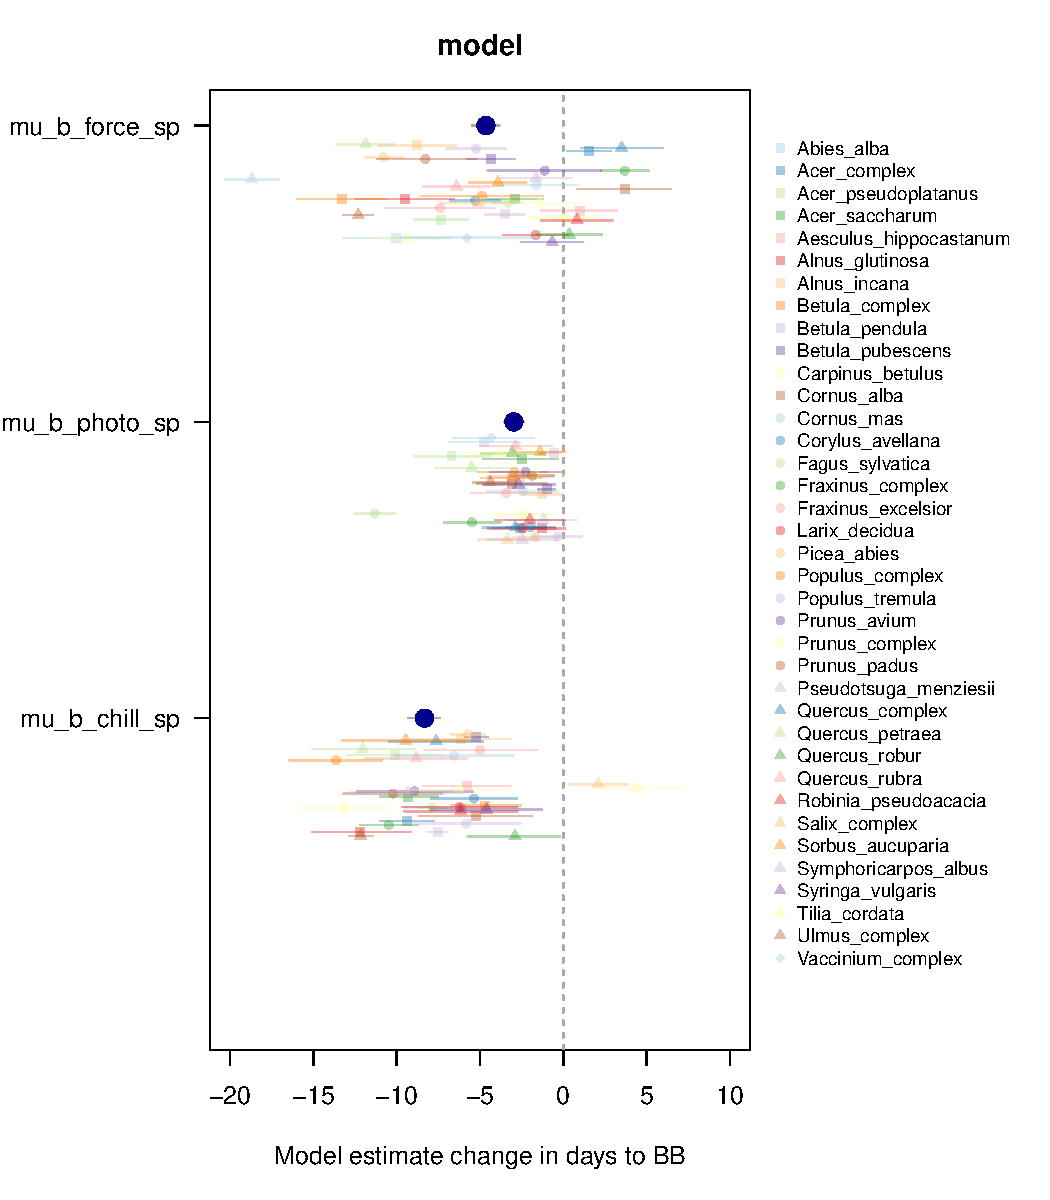
\includegraphics[width=0.75\textwidth]{..//..//analyses/bb_analysis/figures/muplotmodelspcom_expramp_fp_chillports.pdf}
\caption{Budburst model estimates}
\label{fig:mu}
\end{figure}

\begin{figure}[h!]
\centering
\noindent 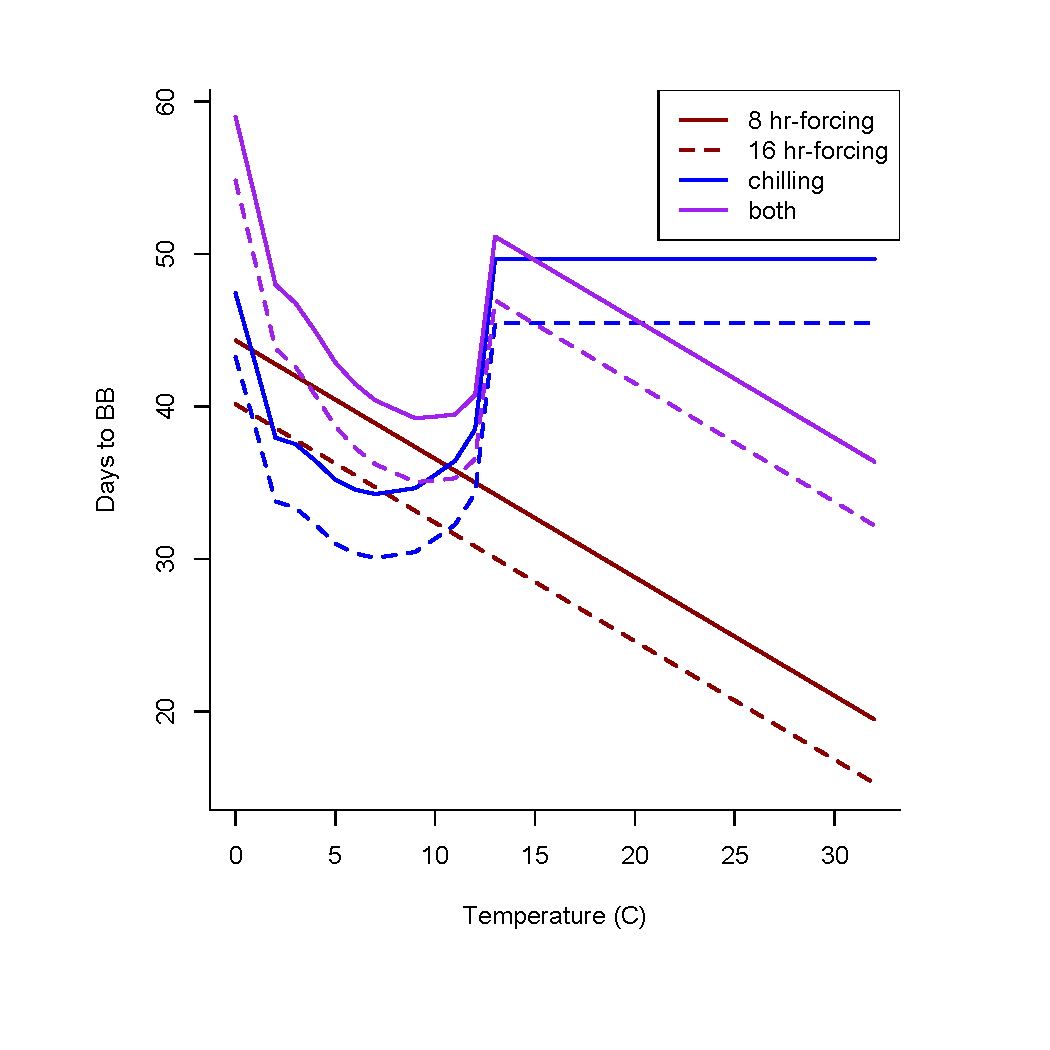
\includegraphics[width=0.75\textwidth]{..//..//analyses/bb_analysis/figures/expcondi_forecastplot.pdf}
\caption{Effects of chilling, forcing, and photoperiod, across the experimental conditions in the OSPREE database. make this part of a 2-panel figure with \ref{fig:mu}. Make a 3D version of this.}
\label{fig:apc}
\end{figure}

\newpage

\begin{figure}[h!]
\centering
\noindent 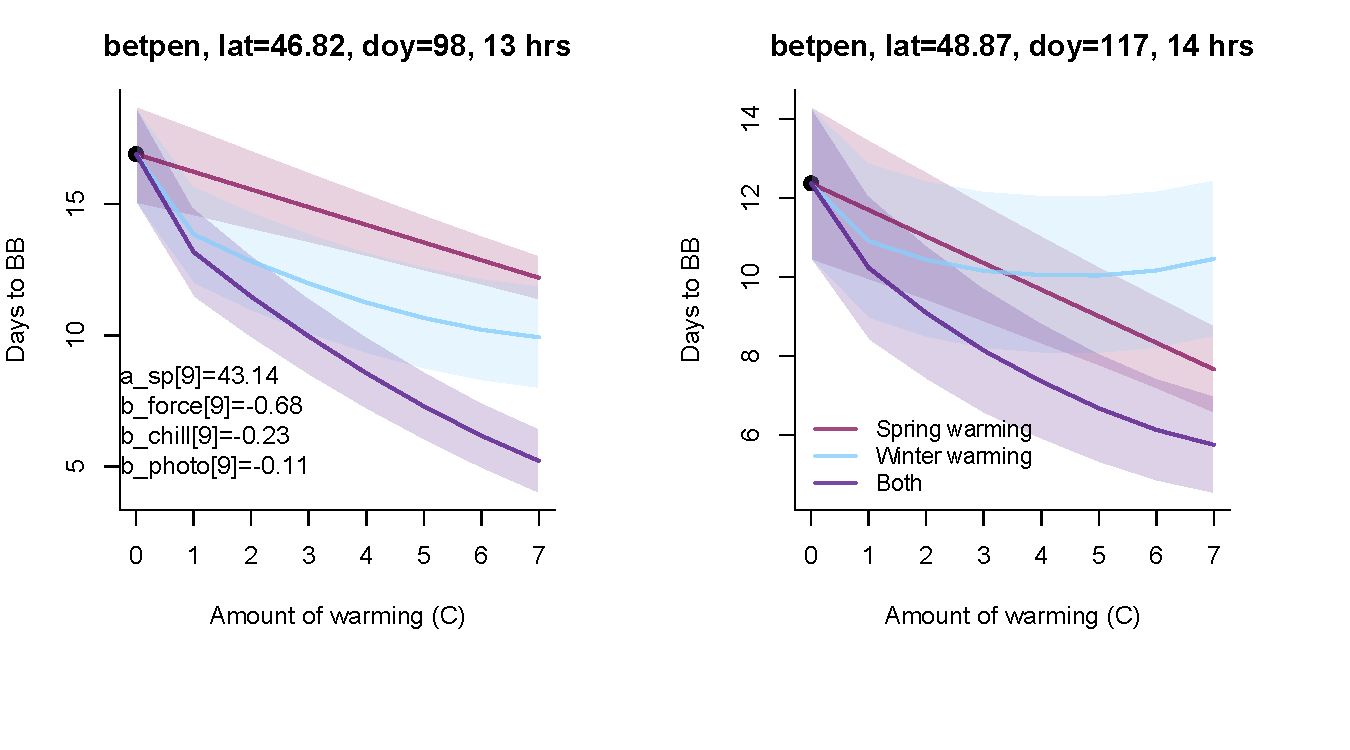
\includegraphics[width=0.75\textwidth]{..//..//analyses/bb_analysis/figures/tempforecast_betpen_minmaxlat_PEPBB_wdl.pdf}
\caption{Implications of global warming on budburst of \emph{Betula pendula} at two locations with differing current climate in Germany, as predicted by our model. Possibly replace with 3D figure? and possibly make a 4-paneled figure with fagsyl}
\label{fig:fore}
\end{figure}
\begin{figure}[h!]
\centering
\noindent 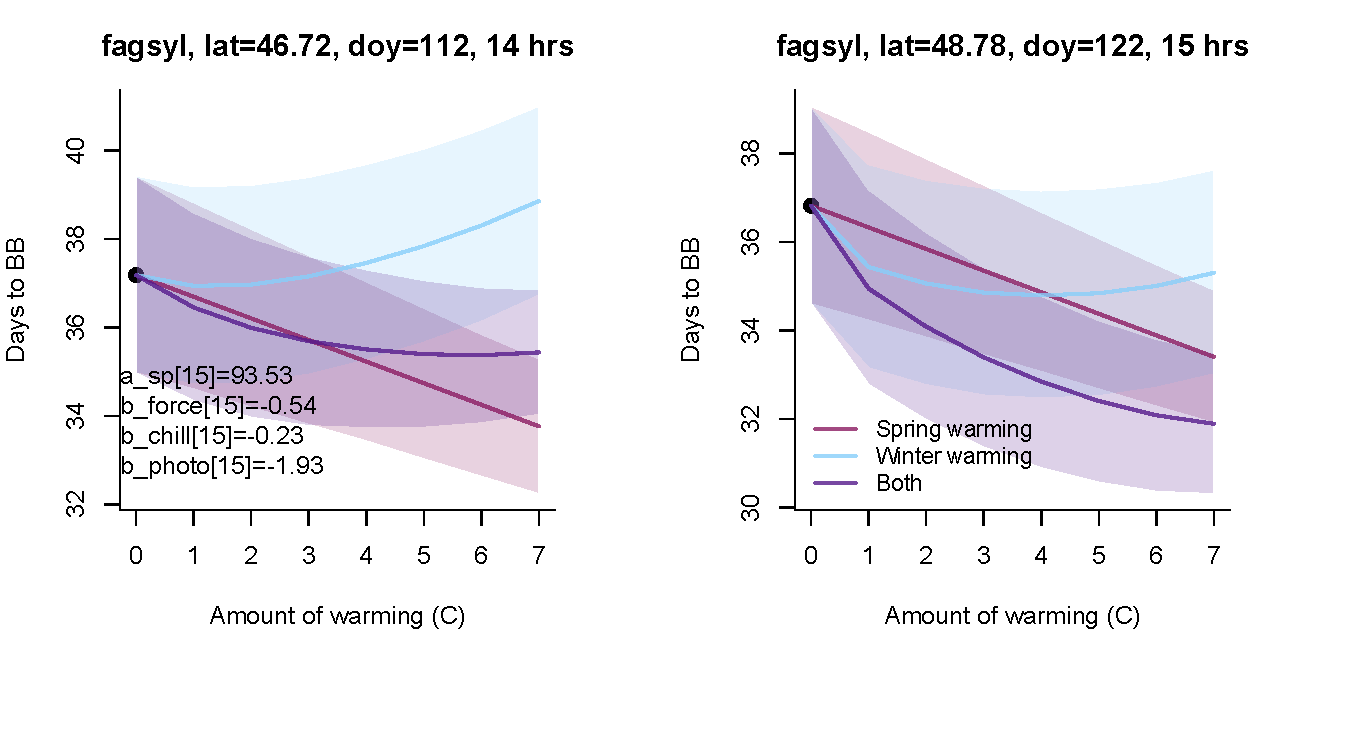
\includegraphics[width=0.75\textwidth]{..//..//analyses/bb_analysis/figures/tempforecast_fagsyl_minmaxlat_PEPBB_wdl.pdf}
\caption{Implications of global warming on budburst of \emph{Fagus sylvatica} at two locations with differing current climate in Germany, as predicted by our model. Possibly replace with 3D figure?}
\label{fig:forefs}
\end{figure}

\newpage
\begin{enumerate}
\item $\mu$ plots


\item  $\mu$ forecasting figures: spring x winter warming -- PEP climate range and experimental climate range
\item Species forecasting with PEP data: \emph{Betula, Fagus} ... need to think on which ones to use (x sites x species focus etc). ... Maybe show photoperiod one?
\item PEP data figure with environmental conditions: as in Cat's figure + OSPREE data + maybe foercasting (at 2C or such?)
\end{enumerate}


{\bf Supplemental figures/tables:}
\begin{enumerate}
\item Map of study locations, shading or symbol coding for number of cues (Lizzie)
\item Map of species forecasting to justify sites
\item Tables, yes.
\item Heat maps for the main data, including by actual study design and by calculated chilling (our calculations)
\item Photoperiod x latitude effects figure
\item Equation of our model

\end{enumerate}
\end{enumerate}

\section{Reference list}

A few categories:\\

Papers about contrasting results over what cues matter from growth chamber studies: \cite{Basler:2012,Basler:2014aa,Caffarra:2011qf,Caffarra:2011a,Caffarra:2011b,Heide:2005aa,koerner2010b,Laube:2014a,vitasse2013,zohner2016}. Get Nanninga \emph{et al.} 2017: 'Increased exposure to chilling advances the time to budburst in North American tree species' and maybe Malyshev \emph{et al.} 2018 `Temporal photoperiod sensitivity and forcing requirements for budburst in temperate tree seedlings.'\\

Papers about declining sensitivities (Ailene will update this list): \cite{Rutishauser:2008,fu2015}. Also look for a Wang \emph{et al.} article `Impacts of global warming on phenology of spring leaf unfolding remain stable in the long run.' Vitasse paper on declining variation across elevation gradient. See \cite{yu2010}, but this is not temperate trees. \\

Papers about chilling units paper (Lizzie gets a list): Fu 2012 from OSPREE. \cite{harrington2015}\cite{lued2011,Luedeling:2011qe,Luedeling2013AgFM}\\

\bibliography{..//..//refs/ospreebibplus.bib}
\end{document}